

\begin{frame}{Mallet}

\begin{itemize}
  \item Developed at UMass Amherst by Andrew McCallum and David Mimno (among others)
  \item Very fast implementation of Gibbs sampling for topic modeling
  \item (Somewhat) friendly interface
  \item Easiest on \textsc{unix}-derived operating systems, but also works on Windows
  \item Requires Java
\end{itemize}

\begin{columns}
\column{.5\linewidth}
\begin{block}{Download Location}
  http://mallet.cs.umass.edu/
\end{block}
\column{.5\linewidth}

\includegraphics[width=.9\linewidth]{topic_models/mallet}
\end{columns}
\end{frame}


\begin{frame}
  \frametitle{Scenario}

  \begin{itemize}
    \item Learn a (small-sized) topic model on \textsc{nsf} data
    \item Apply those topics to \textsc{nrc} data
    \item Discover the priorities of \textsc{nsf}
    \item Connects \textsc{nrc} grants to that model
    \item Walk through the commands to do everything
  \end{itemize}
\end{frame}

\begin{frame}[fragile]


\frametitle {Getting Your Data}

\begin{columns}
  \column{.6\linewidth}
    \begin{itemize}
      \item Text file separated by columns
      \item \alert<1>{First column: doc id}
      \item \alert<2>{Second column: language}
      \item \alert<3>{Third column: text}
    \end{itemize}
  \column{.3\linewidth}
     \begin{tabular}{lll}
       \alert<1>{doc} & \alert<2>{lang} & \alert<3>{text} \\
     \end{tabular}
\end{columns}

\begin{block}{Download}
  \url{http://umiacs.umd.edu/~jbg/lda_demo/nsf-30k.txt}
\end{block}

\pause \pause \pause \pause 
\begin{lstlisting}
doc0    none    It is proposed to grow and characterize ternary alloys of ...
doc1    none    This project will focus on development of new cutting tool designs ...
doc2    none    The purpose of the proposed work is to design a novel cooling device ...
doc3    none    The objective of this research project is to develop a wireless ...
\end{lstlisting}

\end{frame}


\begin{frame}[fragile]

  \frametitle{Preparing \textsc{nsf} Data}

  \begin{block}{Mallet Command}
    mallet \alert<2>{import-file} \alert<3>{--remove-stopwords} \alert<4>{--keep-sequence} \alert<5>{--input ~/data/nsf\_abstracts/nsf-30k.txt} \alert<6>{--output nsf.mallet}
  \end{block}

  \pause

  \begin{itemize}
    \item \alert<2>{Tell Mallet what to do}
    \item \alert<3>{Remove words like ``the'', ``and'', ``of''} (otherwise, they'd be at the top of every topic)
    \item \alert<4>{Remember the order of words} (required for Gibbs sampling)
    \item \alert<5>{The input text file}
    \item \alert<6>{Where it writes the binary file}
  \end{itemize}

\end{frame}

\begin{frame}
  \frametitle{Preparing \textsc{nrc} data}

  \begin{block}{Mallet Command}
    mallet import-file --remove-stopwords --keep-sequence --input ~/data/norwegian\_research/merged.txt --output nrc.mallet \alert<2>{--use-pipe-from nsf.mallet}
  \end{block}

  \begin{itemize}
    \item Nearly identical to previous command
    \pause
    \item Main difference: use \textsc{nsf} vocabulary to encode the data
    \item \textsc{lda} doesn't know what words mean
    \item Internally, these algorithms map words to numbers: oxygen (2134), neutrino (33), Weber (1701)
    \item This ensures that this mapping is consistent between datasets
   \end{itemize}

\end{frame}


\begin{frame}
  \frametitle{Fitting a topic model}

\begin{block}{Mallet Command}
\small
  mallet train-topics --input \alert<2>{nsf.mallet}  --num-topics \alert<3>{10} --num-iterations \alert<4>{100} --output-model \alert<5>{nsf\_10.model} --output-state \alert<6>{nsf\_10.state.gz} --output-doc-topics \alert<7>{nsf\_10.doc} --output-topic-keys \alert<8>{nsf\_10.topics} --inferencer-filename \alert<9>{nsf\_10.inf}
\end{block}

\pause

\begin{columns}

  \column{.65\linewidth}

  \begin{itemize}
    \item The \alert<2>{documents} we learn topics from 
    \item The \alert<3>{number of topics} we'll learn
    \item The \alert<4>{number of sweeps} through data
    \item Save the \alert<5>{resulting model}
    \item Save \alert<6>{Gibbs sampling states}
    \item Save \alert<7>{document-topic associations}
    \item Save \alert<8>{word-topic associations}
    \item Save \alert<9>{inferencer}
  \end{itemize}

  \column{.3\linewidth}
    \only<2>{
\includegraphics[width=0.9\linewidth]{topic_models/newspapers} }
    \only<6>{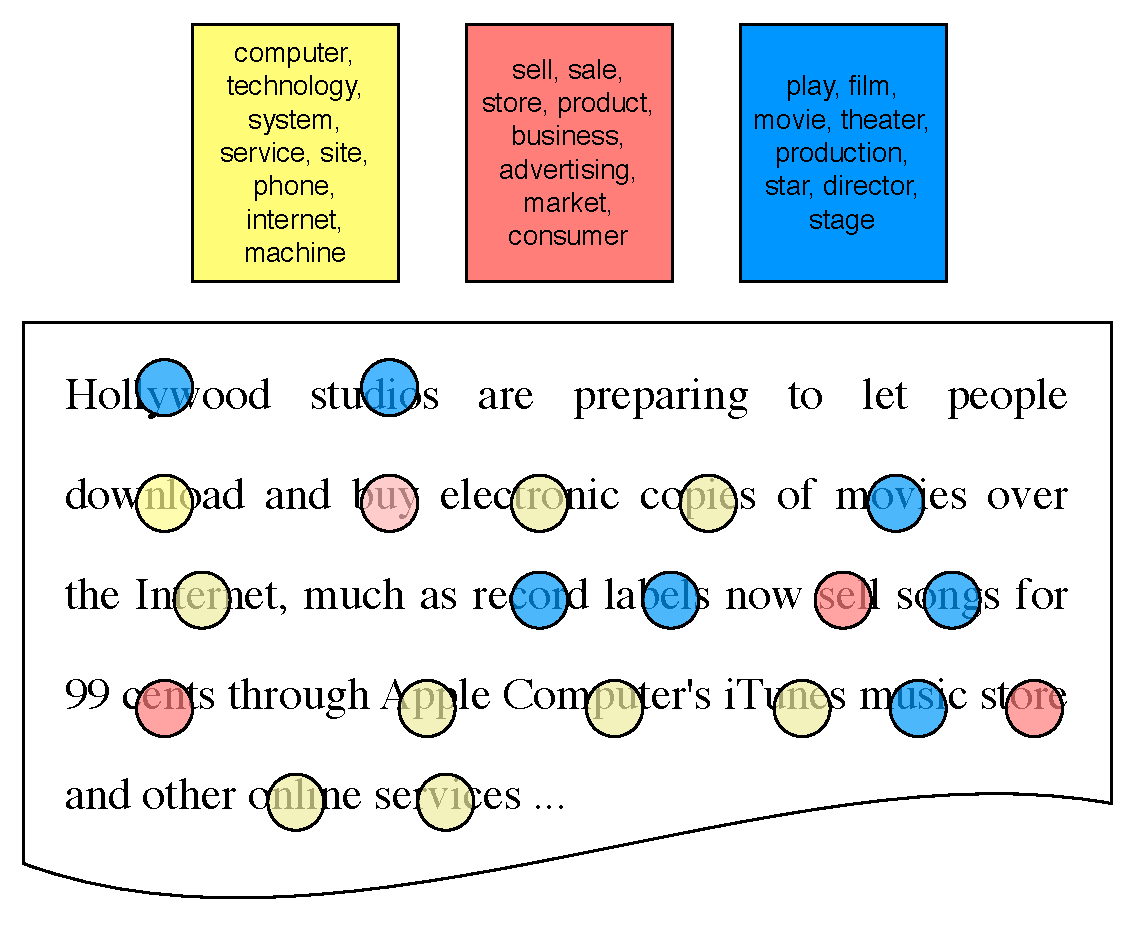
\includegraphics[width=.6\linewidth]{topic_models/inference_3}}
    \only<7>{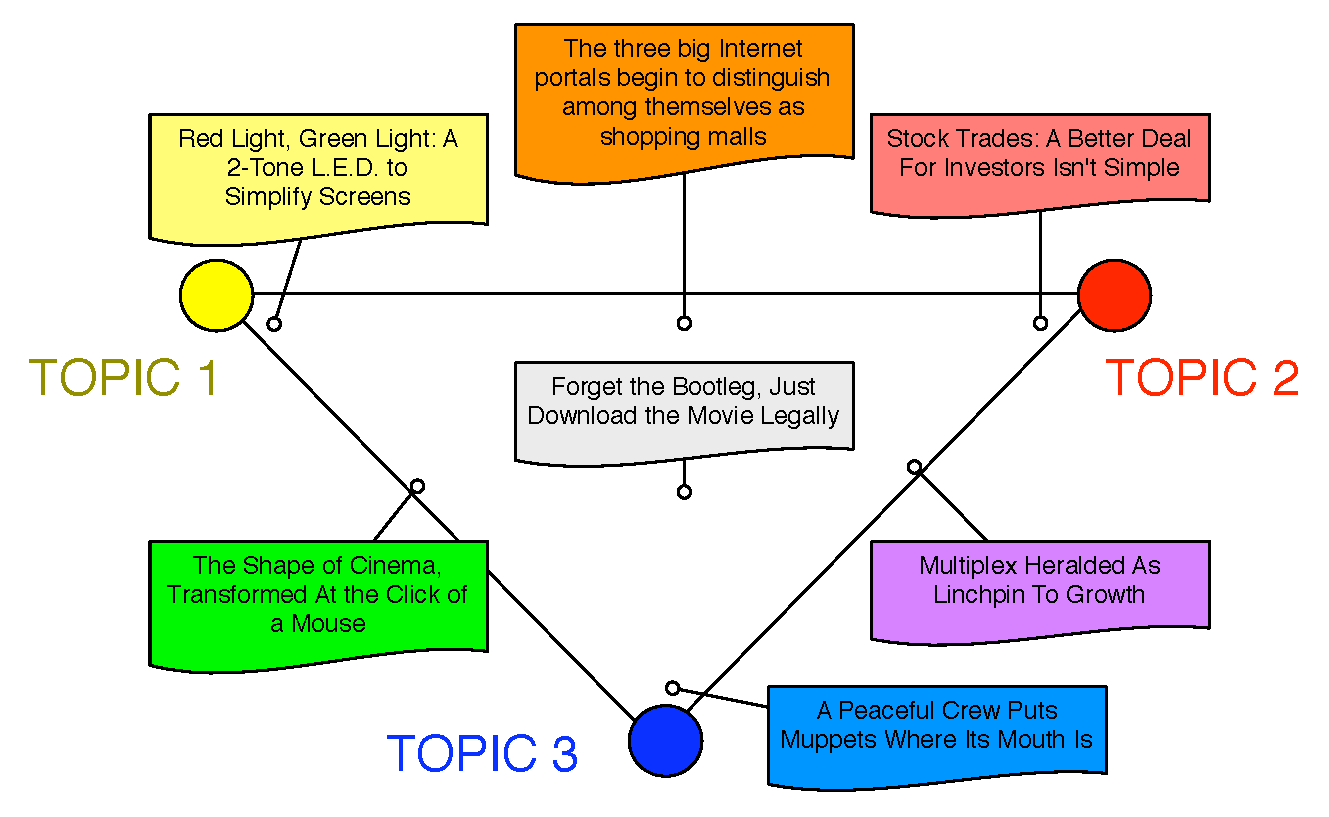
\includegraphics[width=0.9\linewidth]{topic_models/nyt_documents}}
    \only<8>{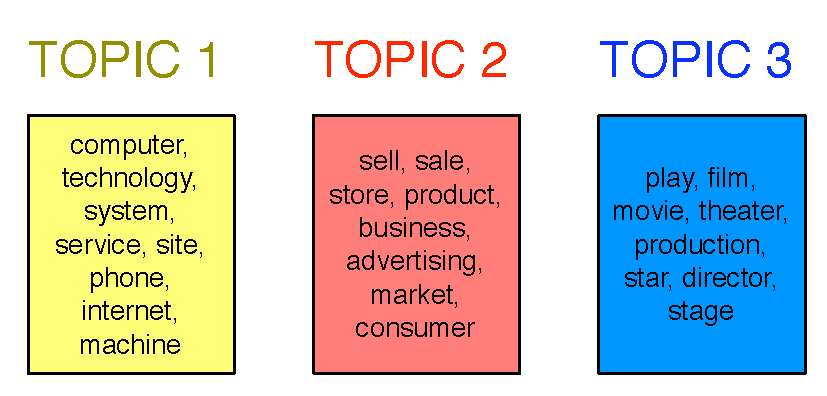
\includegraphics[width=0.9\linewidth]{reading_tea_leaves/figures/nyt_topics_wide}}  
    \only<9>{
    \begin{block}{Inferencer}
        Allows us to apply these topics to another dataset
      \end{block}
    }
  \end{columns}

\end{frame}

\begin{frame}[fragile]
  \frametitle{As Mallet Runs \dots}

  \begin{lstlisting}
<10> LL/token: -10,01271
<20> LL/token: -9,17157
<30> LL/token: -9,01933
<40> LL/token: -8,96692
  \end{lstlisting}

  \begin{itemize}
    \item we want to discover best collection of topics that describes our data
      \item this is defined in terms of probability
        \item stochastic search
          \begin{itemize}
            \item stop when probability levels off
              \item requires thousands of iterations
            \end{itemize}
    \end{itemize}

\end{frame}

\begin{frame}[fragile]
  \frametitle{As Mallet Runs \dots}

  \begin{lstlisting}
0	5	species environmental water natural understanding study research processes climate change ocean global carbon studies production marine important conditions populations effects 
1	5	materials research chemistry properties chemical high magnetic optical surface electron state phase structures structure devices electronic metal molecular studies program 
2	5	systems system design research data control performance network based time applications develop software techniques proposed power application networks developed high 
  \end{lstlisting}

  \begin{itemize}
    \item ID of the topic
    \item Weight of the topic (start the same)
    \item The most probable words in the topic
   \end{itemize}

\end{frame}

\begin{frame}[fragile]
  \frametitle{Word-Topic Association}
  \begin{lstlisting}
0       5       species environmental water natural understanding study research processes climate change ocean global carbon production studies marine populations conditions important long 
1       5       materials research chemistry properties chemical high magnetic optical surface electron phase state structures structure molecular devices electronic metal studies program 
    \end{lstlisting}

    \begin{itemize}
      \item Same information as displayed as Mallet runs
        \item Shows the most probable words in each topic
      \end{itemize}

\end{frame}


\begin{frame}{What topics did we discover?}
\small
  \begin{enumerate}
    \setcounter{enumi}{-1}
    \item {\bf Environmental Science}: climate ocean environmental marine species
    \item {\bf Materials Science}: materials chemistry properties magnetic structure
    \item {\bf Systems Engineering}: control network applications power software
    \item {\bf Social Science}: economic social human policy behavior public
    \item {\bf Training}: undergraduate education program students graduate training
    \item {\bf Physics}: mass energy time flow scale mass rate phase energy
    \item {\bf biology}: cell protein molecular function genes proteins gene cells
    \item {\bf Computer Science}: information web computer research industry
    \item {\bf Geology}: region earth ice provide field sites events mantle deep seismic 
    \item {\bf Math}: theory methods problem mathematical analysis number geometry
    \end{enumerate}
\end{frame}

\begin{frame}[fragile]
  \frametitle{What documents are associated with each topic?}

  \begin{lstlisting}
138     doc138  8       0.291970802919708       4       0.24087591240875914     0
       0.08759124087591241     3       0.072992700729927       7       0.06569343065693431     9       0.051094890510948905    5       0.051094890510948905    1       0.051094890510948905    6       0.043795620437956206    2       0.043795620437956206
139     doc139  4       0.304   5       0.168   6       0.104   9       0.08    8
       0.072   7       0.064   0       0.064   3       0.048   2       0.048   1
       0.048  
    \end{lstlisting}

    \begin{itemize}
      \item Document 138 is associated with topic 4 and topic 8
        \item These are the Training and Geology topics
      \end{itemize}

      \pause

      \vspace{-3cm}

  \begin{block}{doc138}
    \small
This Americas Program award will support a planning visit 
dots  to carry out join research planning with scientists of the Instituto, to investigate field logistics, and examining key field sites, with the goal of developing two joint research projects, as well as a joint training program for advanced students of active tectonics and geologic hazards. The projects include a study of the geodynamic mass balance in the northern Andes between volcanic eruptions and erosion; study of neotectonic deformation and catastrophic sedimentation in the Interandean Valley
  \end{block}

\end{frame}


\begin{frame}
  \frametitle{Applying topics to \textsc{nrc} data}
  \begin{itemize}
    \item Assume that we are satisfied with this topic analysis
    \item \textsc{nsf} is convenient example
      \begin{itemize}
        \item \textsc{eu}-wide research
        \item Wikipedia
        \item Publications
      \end{itemize}
      \item Associate \alert<2>{new documents} with some \alert<3>{standard}
      \item Compare funding levels for comparable topics (regardless of internal classification)
  \end{itemize}

\end{frame}


\begin{frame}
  \frametitle{Applying Topics}
    \begin{block}{Mallet Command}
      mallet infer-topics --input \alert<2>{nrc.mallet} --inferencer \alert<3>{nsf\_10.inf} --output-doc-topics \alert<4>{nrc.doc}
    \end{block}

    \begin{itemize}
      \item Document to apply model to
      \item Inferencer created from model
      \item Output file
    \end{itemize}

\end{frame}

\begin{frame}
  \frametitle{Much more to be done!}

  \begin{itemize}
    \item Bigrams: not all strings separated by spaces are words
      \begin{itemize}
        \item high energy, nano materials, seismic models, undergraduate students
          \item need to be discovered along with topics
        \end{itemize}
        \item Choosing correct granularity
        \item Refining stopword list: investigator, study, research
        \item \alert<2>{Adding constraints}
        \item \alert<2>{Multiple languages}
   \end{itemize}

\end{frame}